\documentclass[a4paper]{article}
\usepackage{amsmath}
\usepackage{amssymb}
\usepackage{braket}%量子力学符号
\usepackage{geometry}
\usepackage{natbib}
\usepackage{float}%稳定图片位置
\usepackage{graphicx,subfig}%画图
\usepackage{caption}
\usepackage[english]{babel}
\usepackage{indentfirst}%缩进
\usepackage{enumerate}%加序号
\usepackage{multirow}%合并行
\usepackage{hyperref}
\usepackage{verbatim}
\title{\Large \textbf{VP390 Problem Set 8}\\
\author{\textbf{Pan, Chongdan ID:516370910121}\\
}
}
\begin{document}
\maketitle
\section{Problem 1}
\noindent
$\braket{v^2}=\int_0^{\infty}v^2f(v)\mathrm{d}v=\int_0^{\infty}4\pi v^4(\frac{m}{2\pi k_BT})^{3/2}\exp(-\frac{mv^2}{2k_BT})\mathrm{d}v=\int_0^{\infty}v^2f(E)\mathrm{d}E=\int_0^{\infty}\frac{2E}{m}f(E)\mathrm{d}E$
$$\textbf{Pr}(\ket{0}^{\bigotimes n-1})=|\frac{1}{2^n}\sum_{x=0}^{2^{n-1}}(-1)^{f(x)}|^2$$
\\$\braket{v^2}=\frac{2}{m}\braket{E}=\frac{3}{m}k_BT$
\section{Problem 2}
\noindent
\begin{enumerate}[(a)]
    \item We can use the Maxwell distribution for the energy: 
    \\$n(E_i)=2^{(i+1)(i+2)/2}\frac{1}{Z}\exp(-\frac{E_i}{k_BT})$
    \\$\frac{n(E_3)}{n(E_1)}=\frac{1024}{3}\exp(-12.1/0.026)\approx0$
    \\$\frac{n(E_2)}{n(E_1)}=\frac{64}{3}\exp(-10.2/0.026)\approx0$
    \item $Z=\sum_i e^{-E_i/k_BT}\approx e^{-E_1/k_BT}+e^{-E_2/k_BT}+e^{-E_3/k_BT}$
    \\Assume $k_BT=\alpha$, then $Z=\frac{1}{e^{13.6/\alpha}+e^{3.4/\alpha}+e^{1.5/\alpha}}$
    \\$f_B(E_2)=\frac{e^{3.4/\alpha}}{e^{13.6/\alpha}+e^{3.4/\alpha}+e^{1.5/\alpha}}=0.01\rightarrow\alpha=2.22\rightarrow T\approx 25784K$
    \item $f(E_3)=\frac{e^{1.5/\alpha}}{e^{13.6/\alpha}+e^{3.4/\alpha}+e^{1.5/\alpha}}\approx4\times10^{-3}$
\end{enumerate}
\section{Problem 3}
\noindent
\begin{enumerate}[(a)]
    \item $f(u)\mathrm{d}u=C\exp(-\frac{Au^2}{k_BT})\mathrm{d}u$
    \\$\int_{-\infty}^\infty f(v)\mathrm{d}v=\int_{-\infty}^\infty C\exp(-\frac{Au^2}{k_BT})\mathrm{d}u=C\sqrt{\frac{\pi k_BT}{A}}=1$
    \\$C=\sqrt{\frac{A}{\pi k_BT}}$
    \item $\braket{E}=\braket{Au^2}=\int_{-\infty}^\infty Au^2\sqrt{\frac{A}{\pi k_BT}}\exp(-\frac{Au^2}{k_BT})\mathrm{d}u$
    \\$2A\sqrt{\frac{A}{\pi k_BT}}\int_0^\infty u^2\exp(-\frac{Au^2}{k_BT})\mathrm{d}u=2A\sqrt{\frac{A}{\pi k_BT}}\frac{1}{4}\sqrt{\pi}(\frac{A}{k_BT})^{-\frac{3}{2}}=\frac{1}{2}k_BT$
\end{enumerate}
\section{Problem 4}
\noindent When under same conditions, compared to classic particles, fermions will be affected by an extra pressure due to the Pauli repulsion. Therefore, fermions gases will have a higher pressure.
\section{Problem 5}
We can only use the Boltzmann distribution when $\frac{h}{\sqrt{3mk_BT}}(\frac{N}{V})^{1/3}<<1$
\\$PV=NTR\rightarrow\frac{N}{V}=\frac{P}{TR}\rightarrow\frac{6.63\times10^{-34}}{\sqrt{3\times2.02\times1.66\times10^{-27}\times1.38\times10^{-23}T}}(\frac{101325}{8.314T})^{1/3}=1$
\\$4.09\times10^{-8}T^{-5/6}=1\rightarrow T=1.36\times10^{-9 }K$
\section{Problem 6}
\noindent \begin{enumerate}[(a)]
    \item For copper, $\braket{E}=\frac{3}{5}E_F=\frac{3}{5}\times7.06=4.236\text{eV}$
    \item For lithium, $\braket{E}=\frac{3}{5}E_F=\frac{3}{5}\times4.77=2.862\text{eV}$
\end{enumerate}
\section{Problem 7}
\begin{figure}[H]
    \centering
    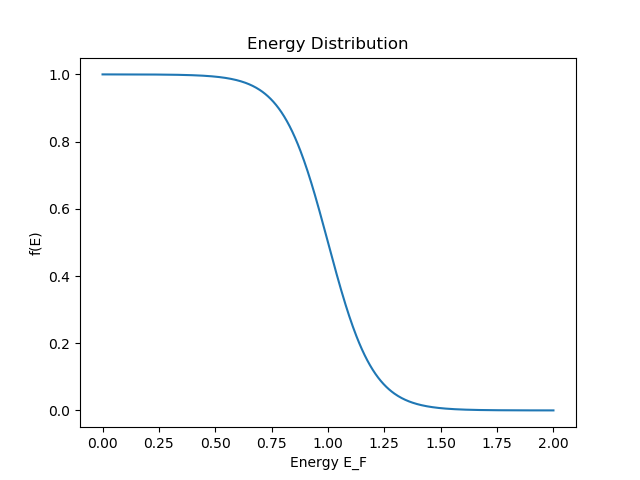
\includegraphics[scale=0.4]{P1.png}
    \caption{$f_{FD}(E)$ vs. $E$ when $T=0.1T_F$}
\end{figure}
\begin{figure}[H]
    \centering
    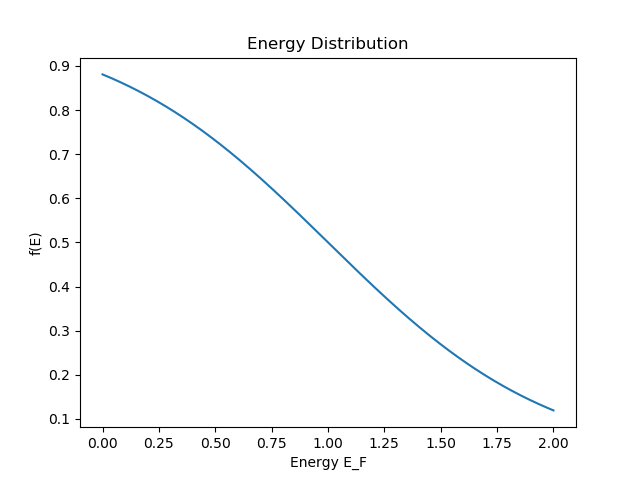
\includegraphics[scale=0.4]{P2.png}
    \caption{$f_{FD}(E)$ vs. $E$ when $T=0.5T_F$}
\end{figure}
\section{Problem 8}
\noindent
The fermi energy for Silver is 5.49eV and the corresponding fermi temperature is $6.38\times10^4K$
\\$k_BT=8.617\times10^{-5}\times300=0.02585\text{eV}<<5.49$
\\$\int_{E_F}^\infty f_{FD}(E)\mathrm{d}E=\int_{5.49}^\infty\frac{1}{e^{(E-5.49)/0.02585}+1}\mathrm{d}E=0.02585\ln(2)=0.0179$
\\$\int_{0}^\infty f_{FD}(E)\mathrm{d}E=\int_{0}^\infty\frac{1}{e^{(E-5.49)/0.02585}+1}\mathrm{d}E=0.02585\ln(e^{(5.49/0.02585)}+1)=5.49$
\\The percentage is $\frac{0.0179}{5.49}\approx0.003=0.3\%$
\section{Problem 9}
\noindent
\begin{enumerate}[(a)]
    \item For 2D, $N=\frac{1}{4}\pi R^2=\frac{\pi}{4}(\frac{E}{E_0})$
    \\$g(E)=\frac{\mathrm{d}N}{\mathrm{d}E}=\frac{\pi}{4E_0}=\frac{mL^2}{2\hbar^2\pi}$
    \\Since the particle is electron $g_e(E)=2g(E)=\frac{mL^2}{\hbar^2\pi}$
    \item For 1D, $N=\frac{1}{2}R=\frac{1}{2}\sqrt{\frac{E}{E_0}}$
    \\$g(E)=\frac{\mathrm{d}N}{\mathrm{d}E}=\frac{1}{4}\sqrt{\frac{2mL^2}{\hbar^2\pi^2E}}$
    \\Since the particle is electron $g_e(E)=2g(E)=\frac{1}{2}\sqrt{\frac{2mL^2}{\hbar^2\pi^2E}}$
\end{enumerate}
\section{Problem 10}
\noindent $\frac{N}{L}=(8.61\times10^28)^{1/3}\approx 4.42\times10^9$/m
\\$E_F=\frac{h^2}{32m}(\frac{N}{L})^2=\frac{(6.63\times10^{-34})^2}{32\times9.11\times10^{-31}}(4.42\times10^9)^2\approx1.84$eV
\end{document}